
\begin{frame}{Sự phụ thuộc của chất lượng ảnh vào các tham số của mô hình}

\begin{figure}[htp]
        \centering
        \begin{tabular}{@{}c@{\hspace{0.1em}}c@{\hspace{0.1em}}c@{\hspace{0.1em}}c@{\hspace{0.1em}}c@{\hspace{0.1em}}c@{\hspace{0.1em}}c@{\hspace{0.1em}}c@{}}
             \includegraphics[width=0.12\linewidth]{Figures/cfg/tiger1.png} & 
             \includegraphics[width=0.12\linewidth]{Figures/cfg/tiger3.png} & 
             \includegraphics[width=0.12\linewidth]{Figures/cfg/tiger5.png} & 
             \includegraphics[width=0.12\linewidth]{Figures/cfg/tiger7.png} & 
             \includegraphics[width=0.12\linewidth]{Figures/cfg/tiger9.png} & 
             \includegraphics[width=0.12\linewidth]{Figures/cfg/tiger11.png} & 
             \includegraphics[width=0.12\linewidth]{Figures/cfg/tiger13.png} & 
             \includegraphics[width=0.12\linewidth]{Figures/cfg/tiger15.png} \\ [-3pt]   
             
             hd = 1 & 
             hd = 3 & 
             hd = 5 & 
             hd = 7 & 
             hd = 9 & 
             hd = 11 & 
             hd = 13 & 
             hd = 15 
                 
        \end{tabular}
        % \caption{Ảnh so sánh các kết quả khi thay đổi giá trị của hệ số hướng dẫn (hd) của lời nhắc văn bản.}
        % \label{fig:cfgsample}
    \end{figure}
    
    \begin{figure}[htp]
    	\centering
    	\begin{tabular}{@{}c@{\hspace{0.1em}}c@{\hspace{0.1em}}c@{\hspace{0.1em}}c@{\hspace{0.1em}}c@{}}
    		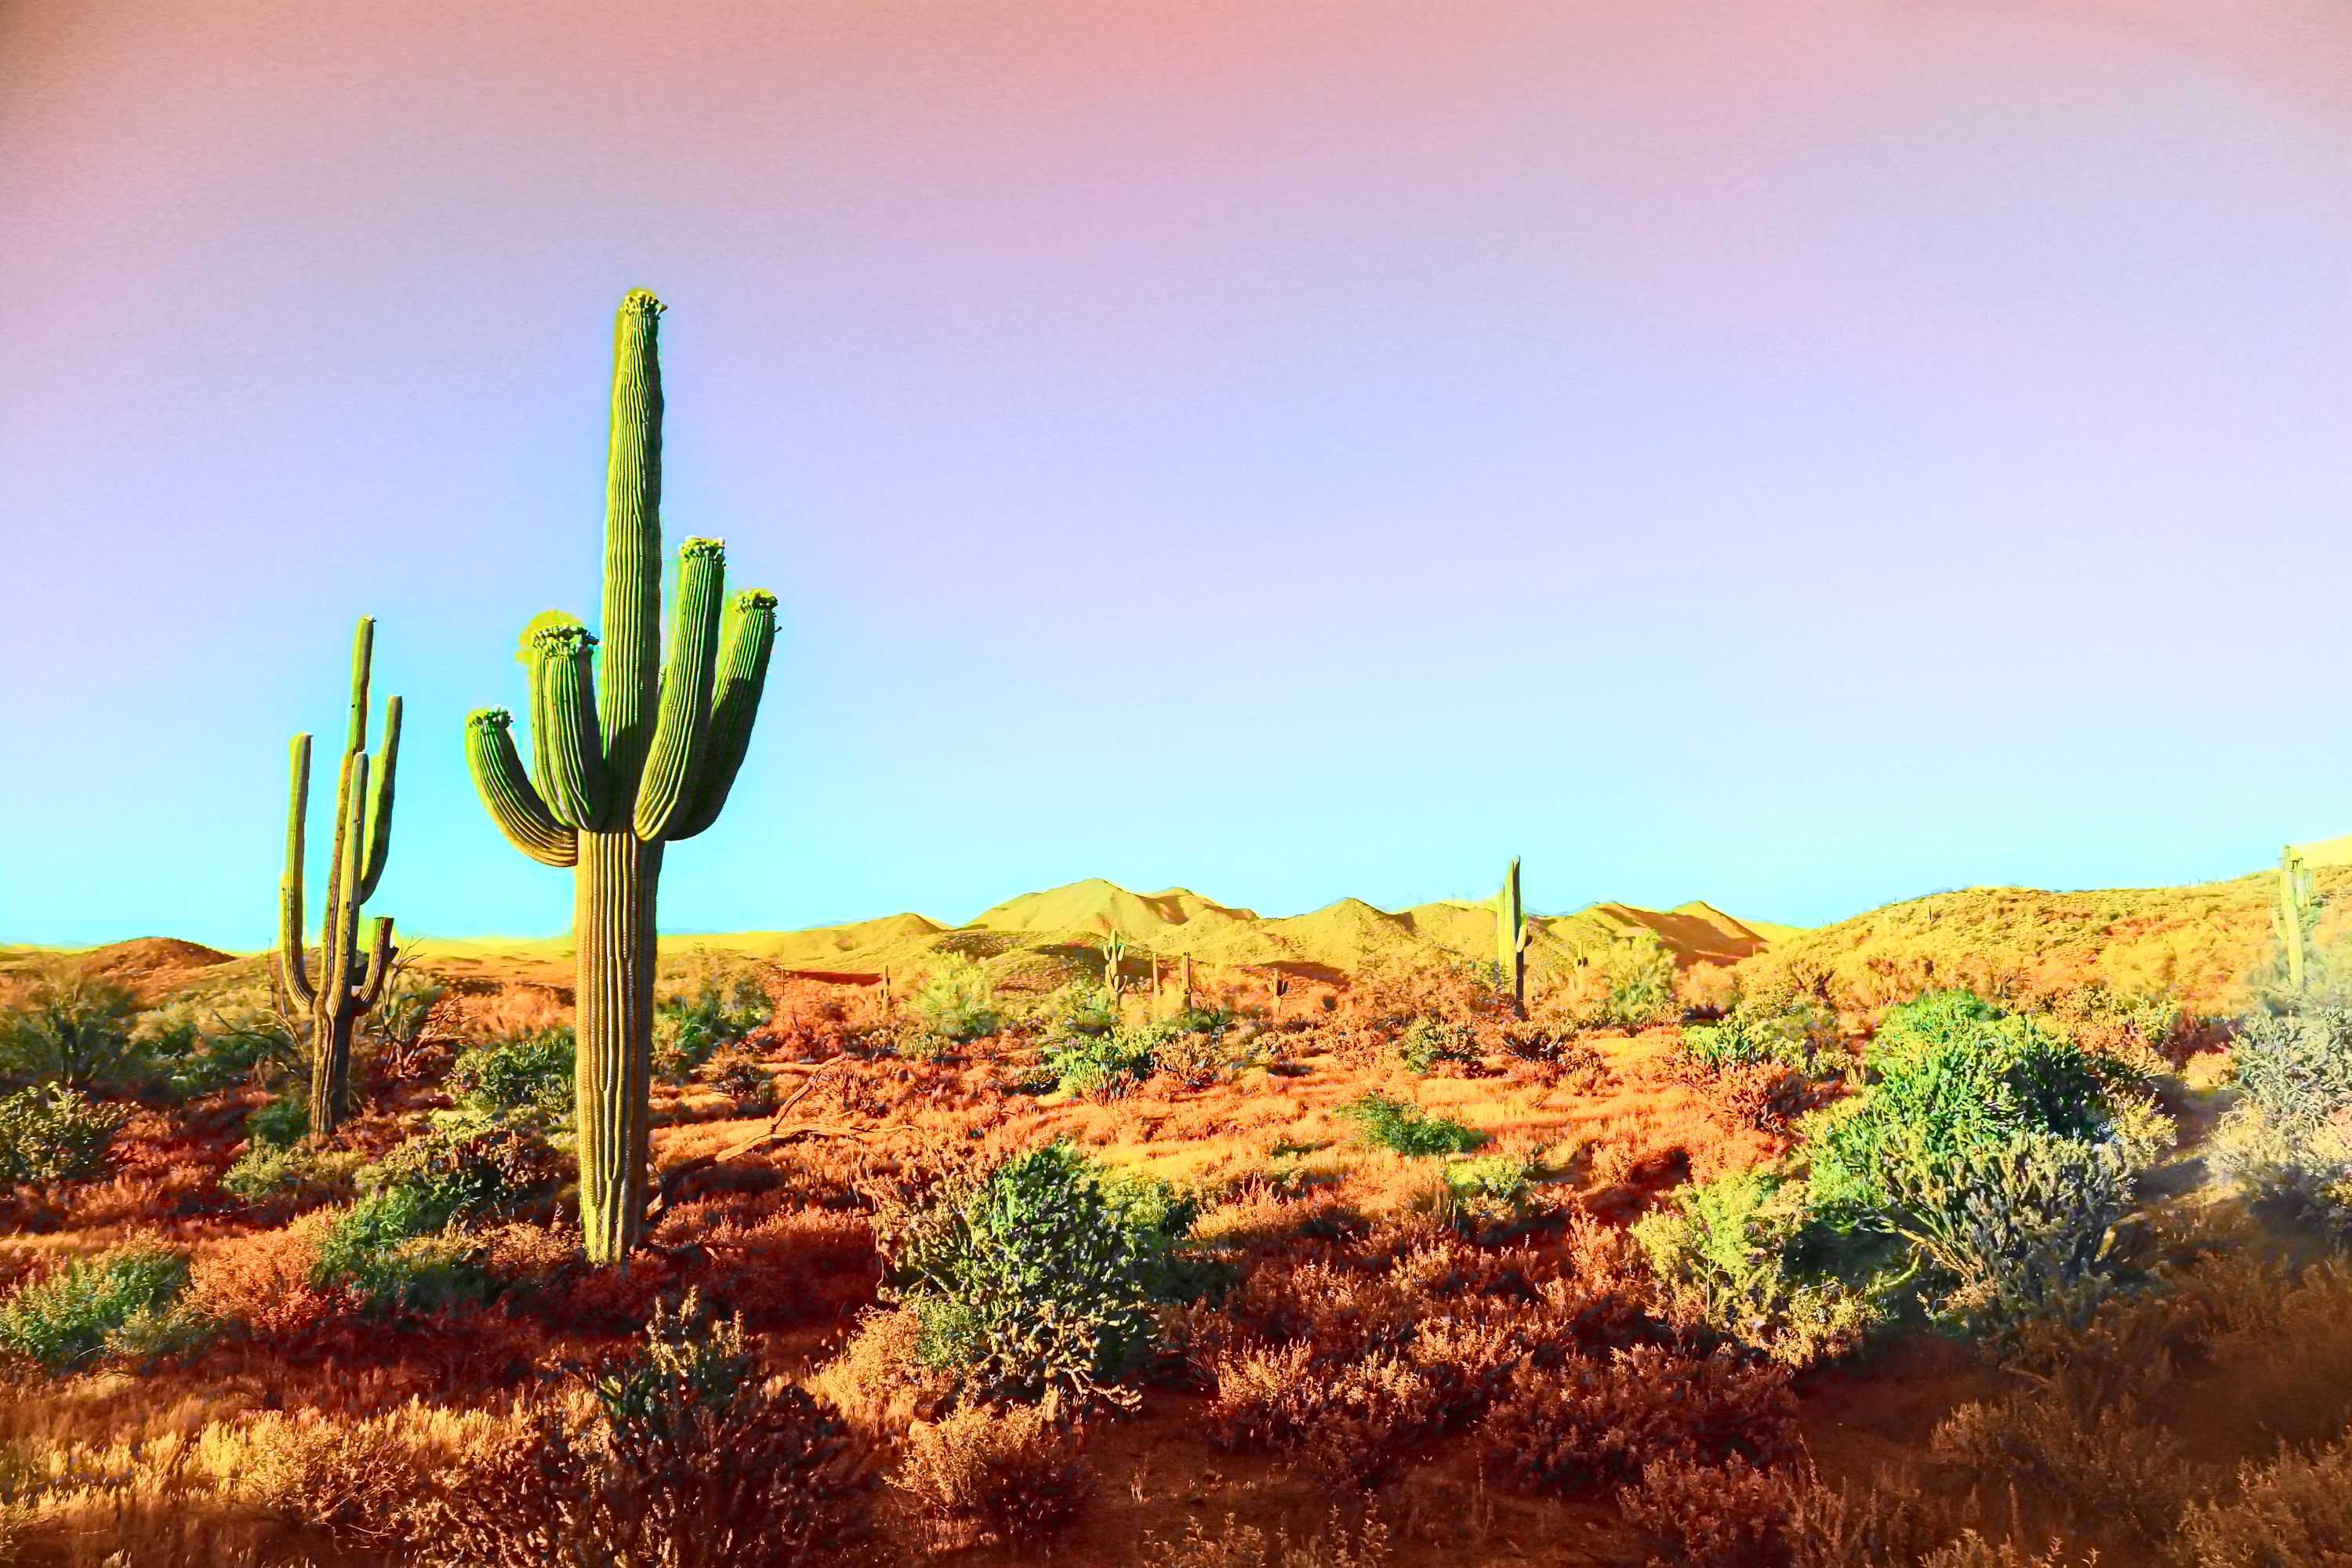
\includegraphics[width=0.19\linewidth]{Figures/step/10.png} & 
    		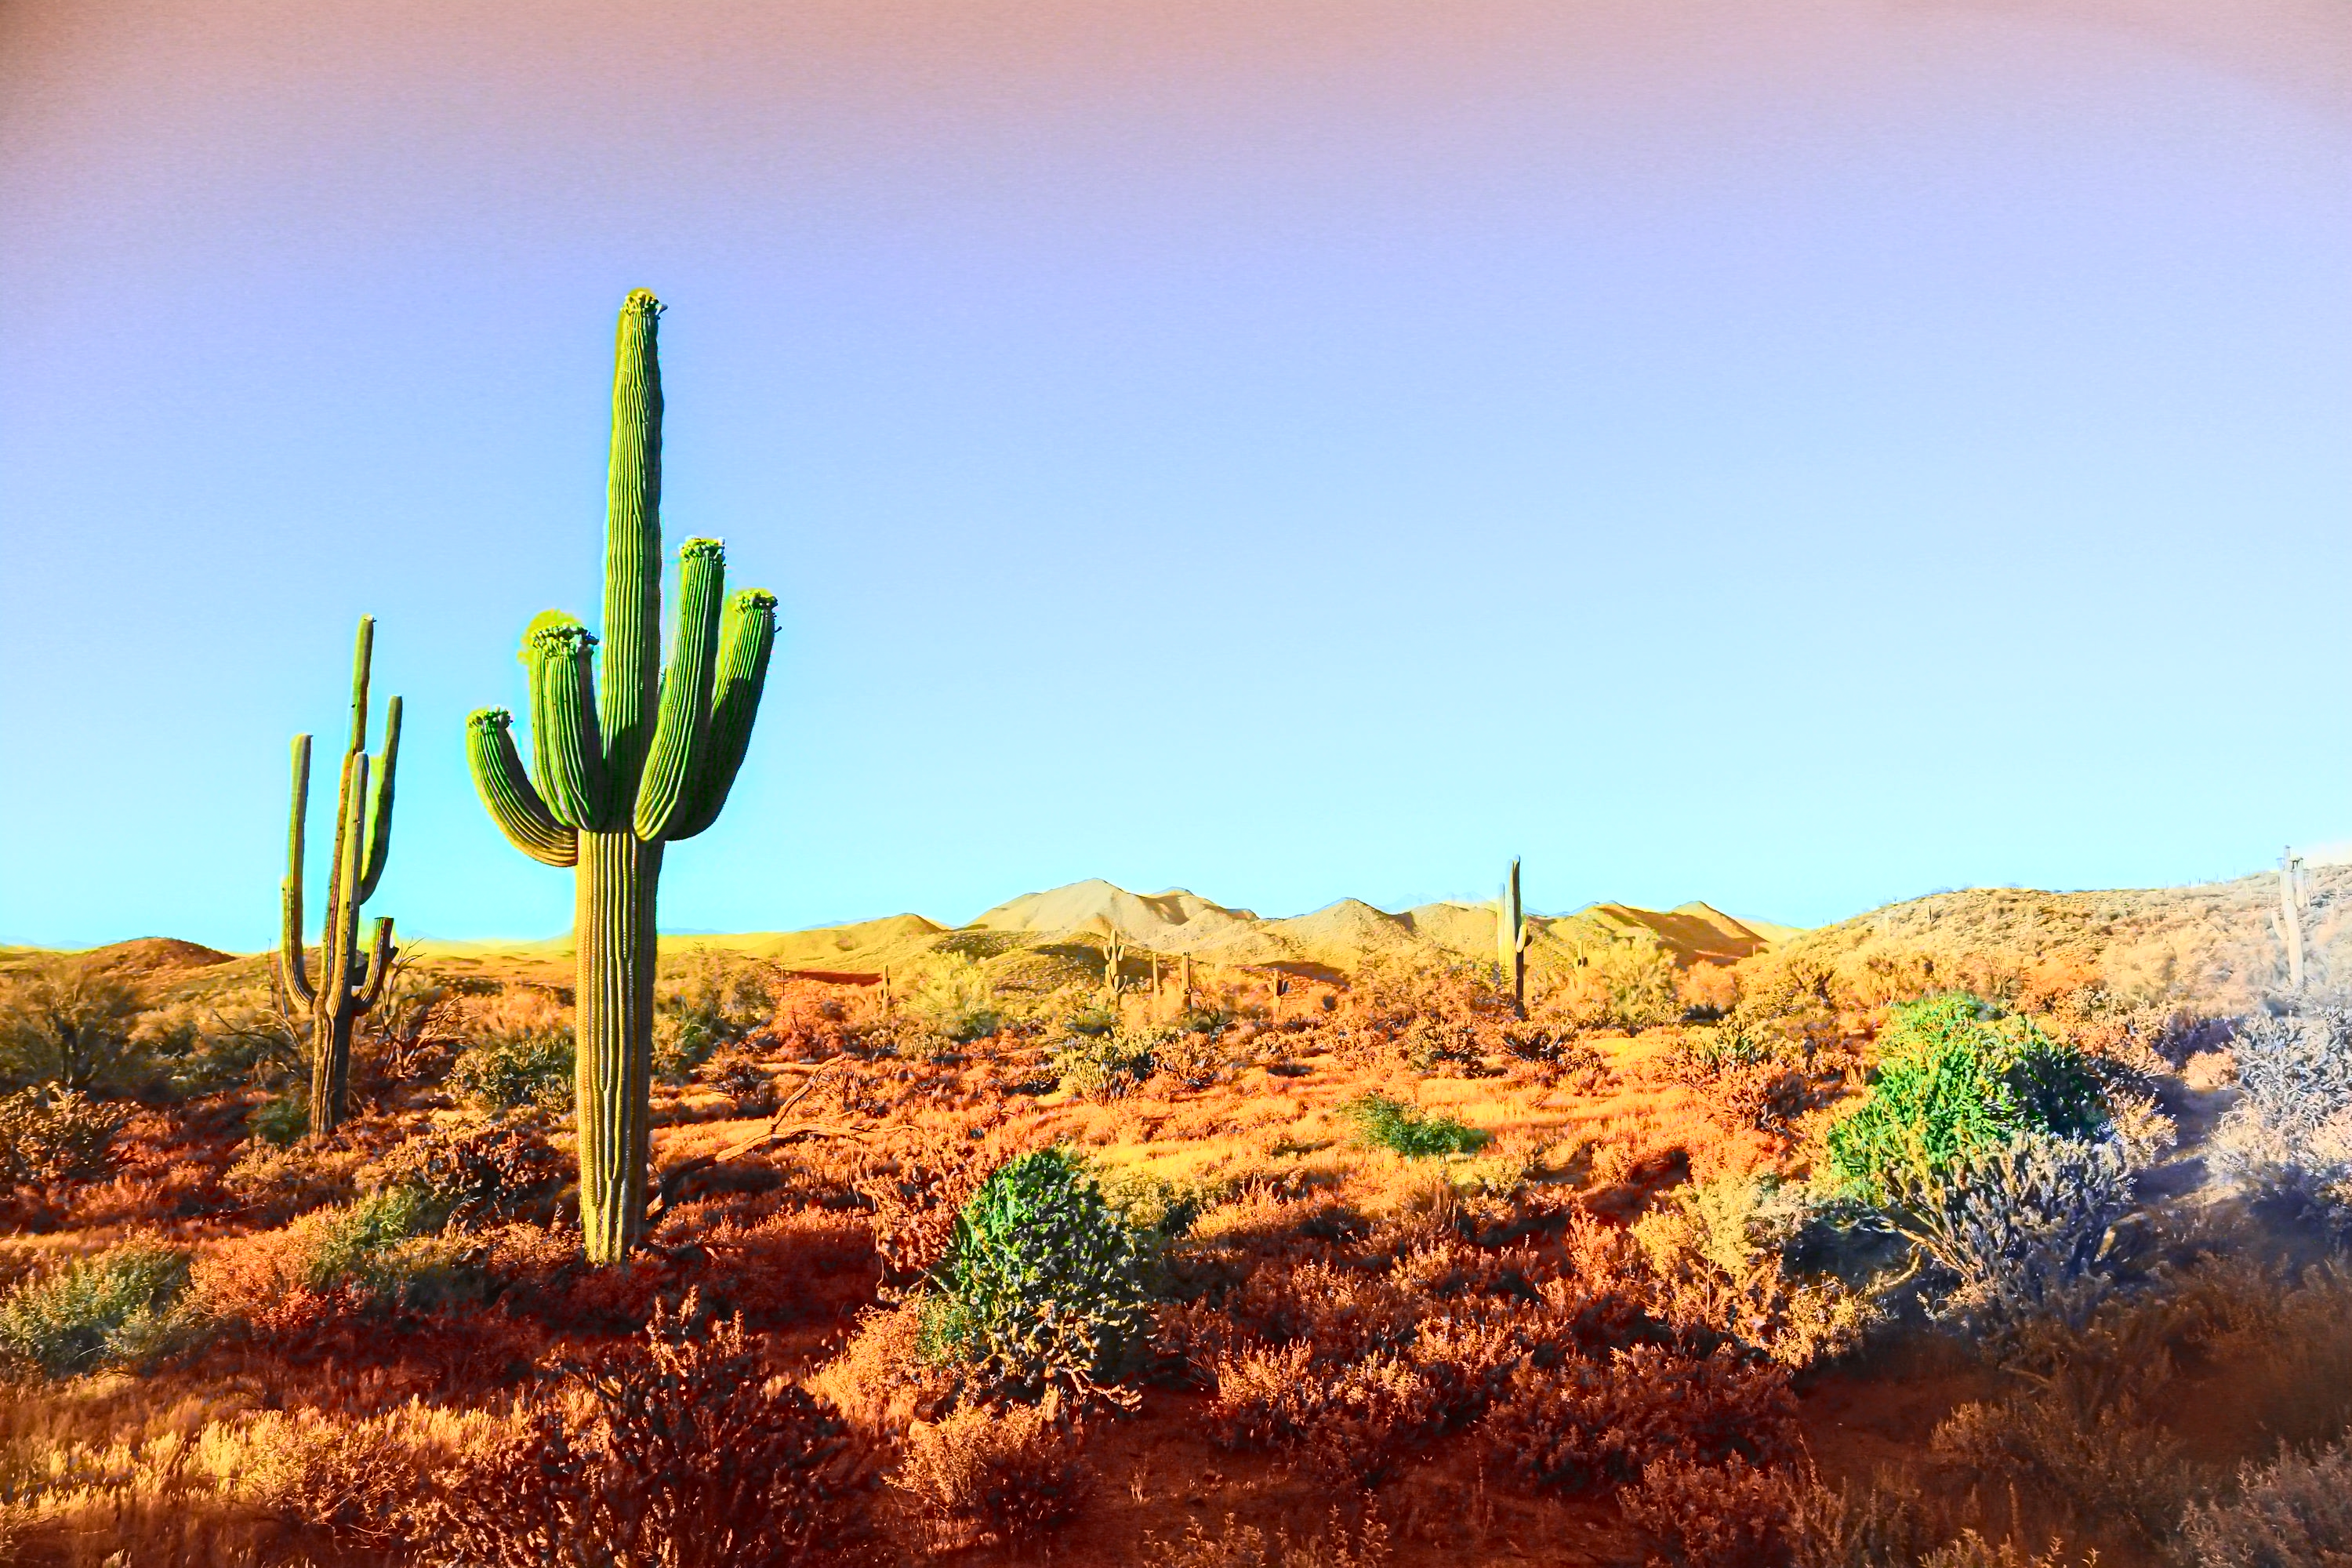
\includegraphics[width=0.19\linewidth]{Figures/step/20.png} & 
    		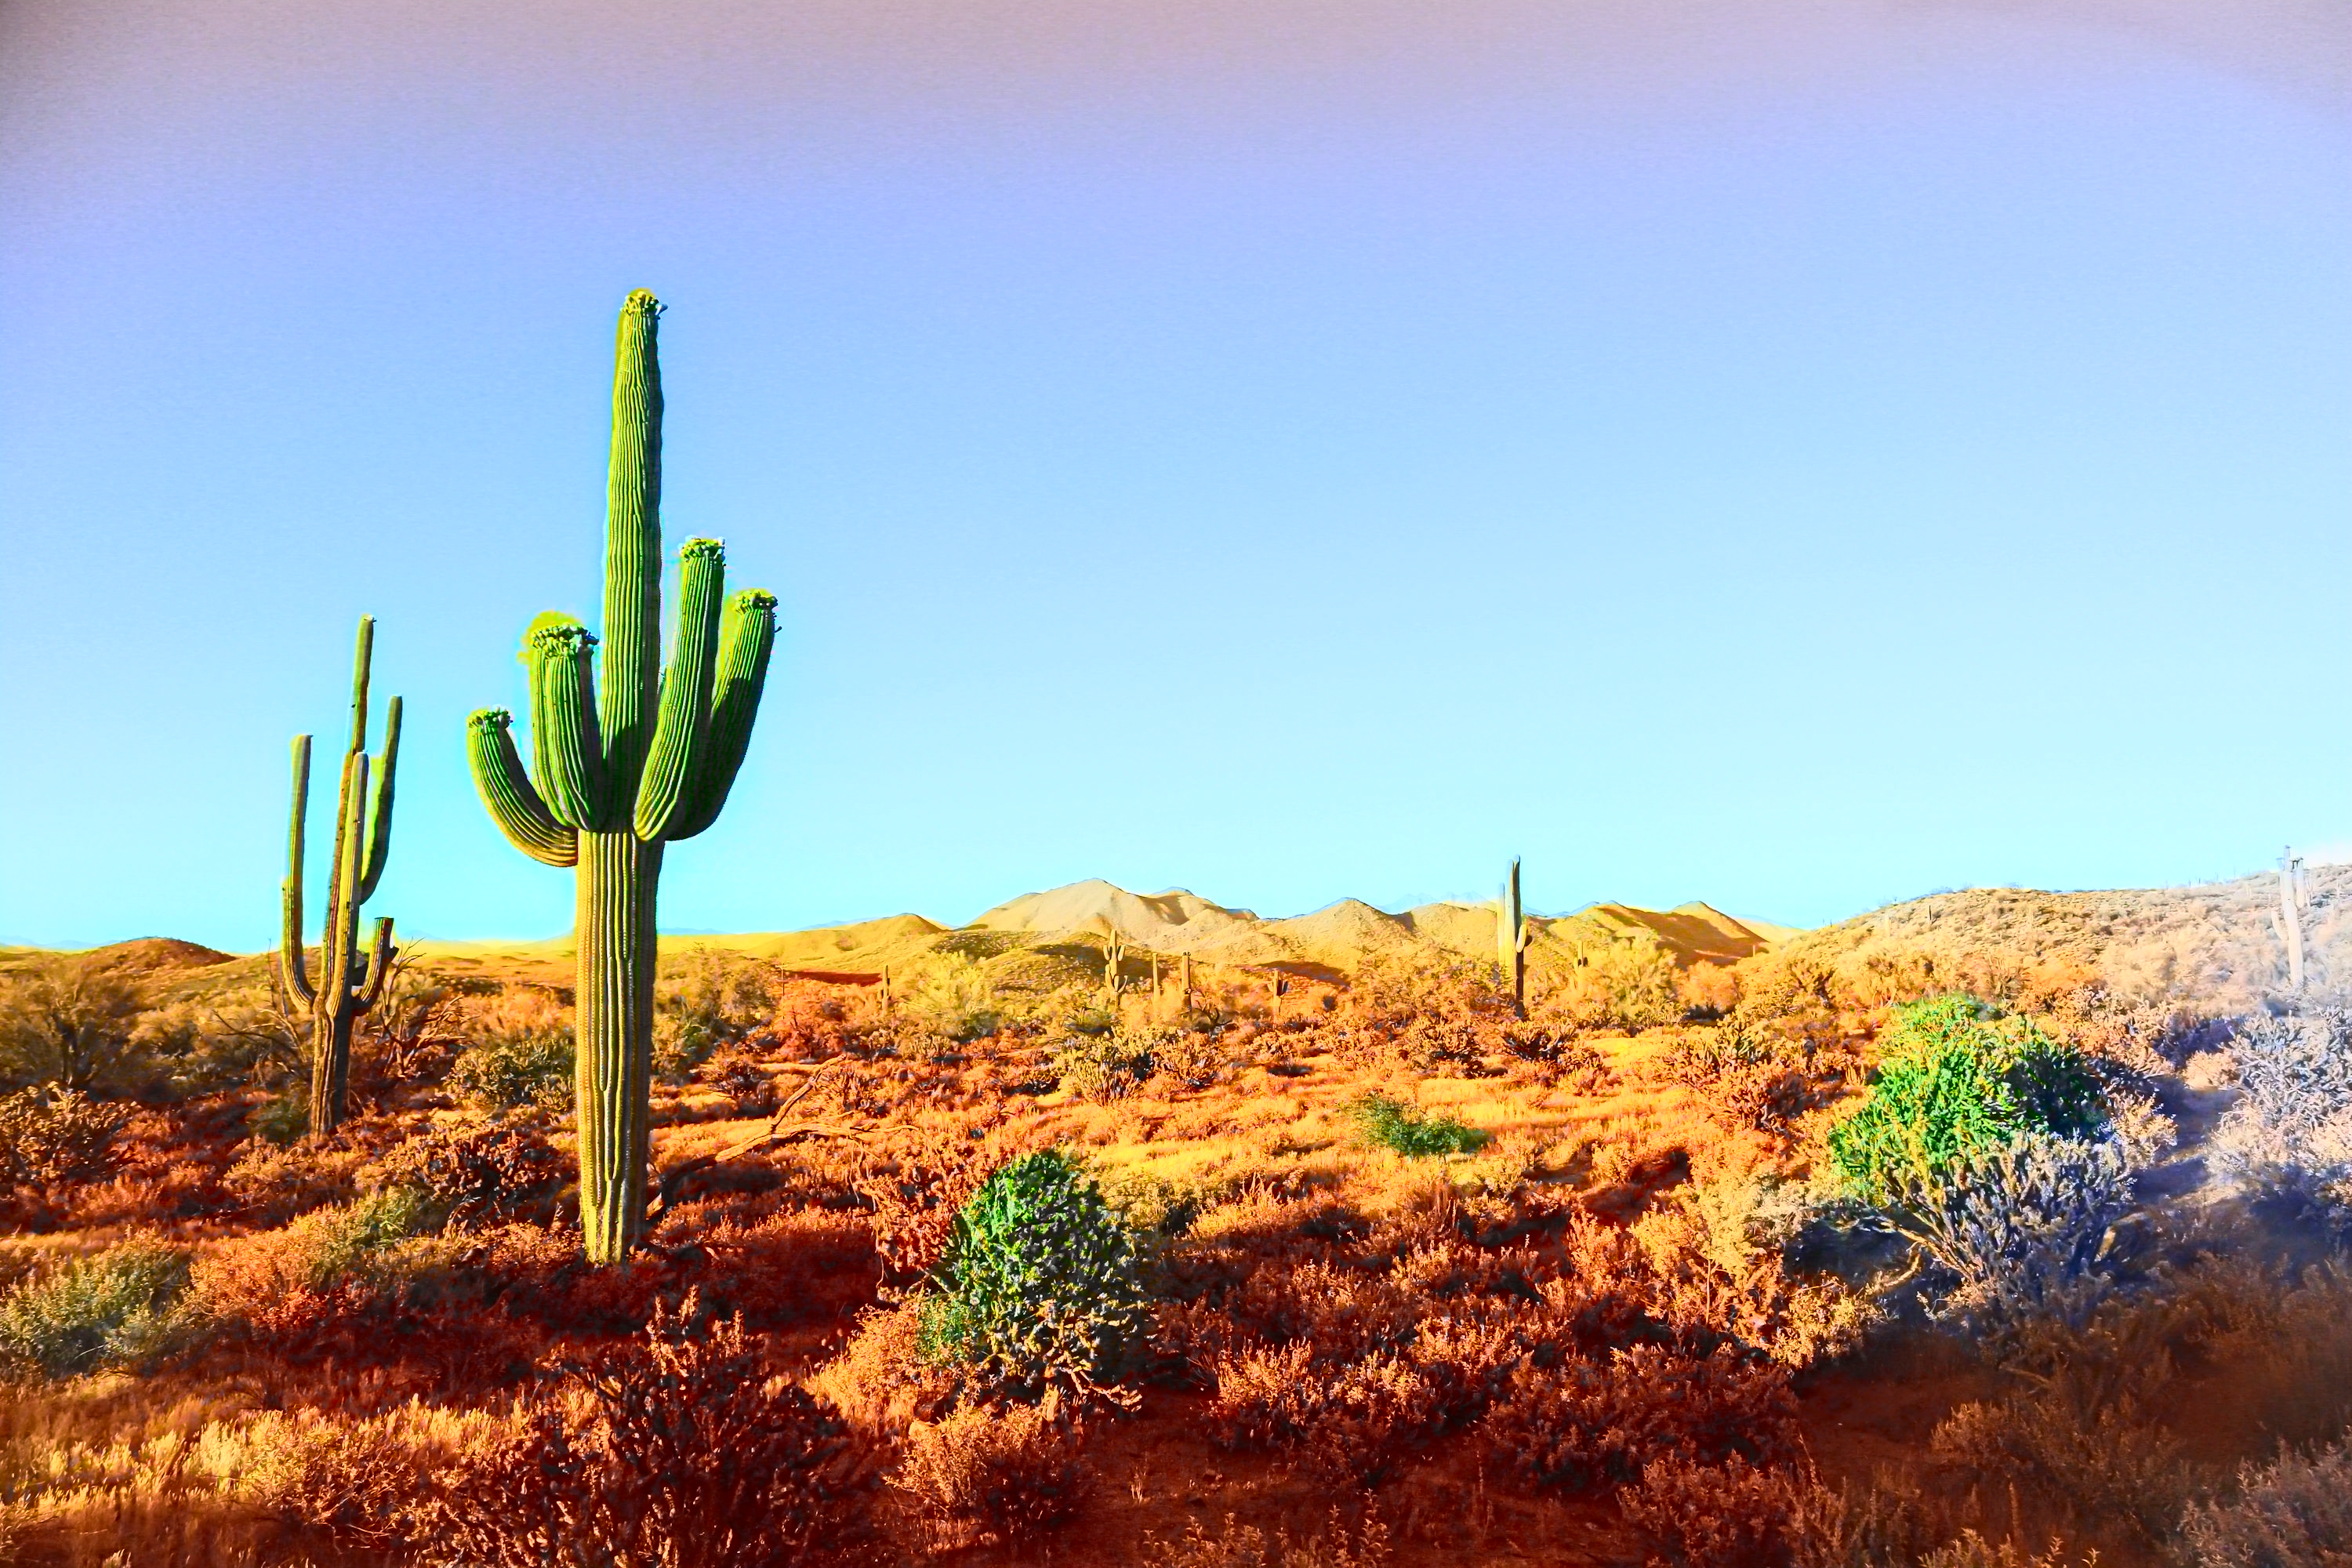
\includegraphics[width=0.19\linewidth]{Figures/step/30.png} & 
    		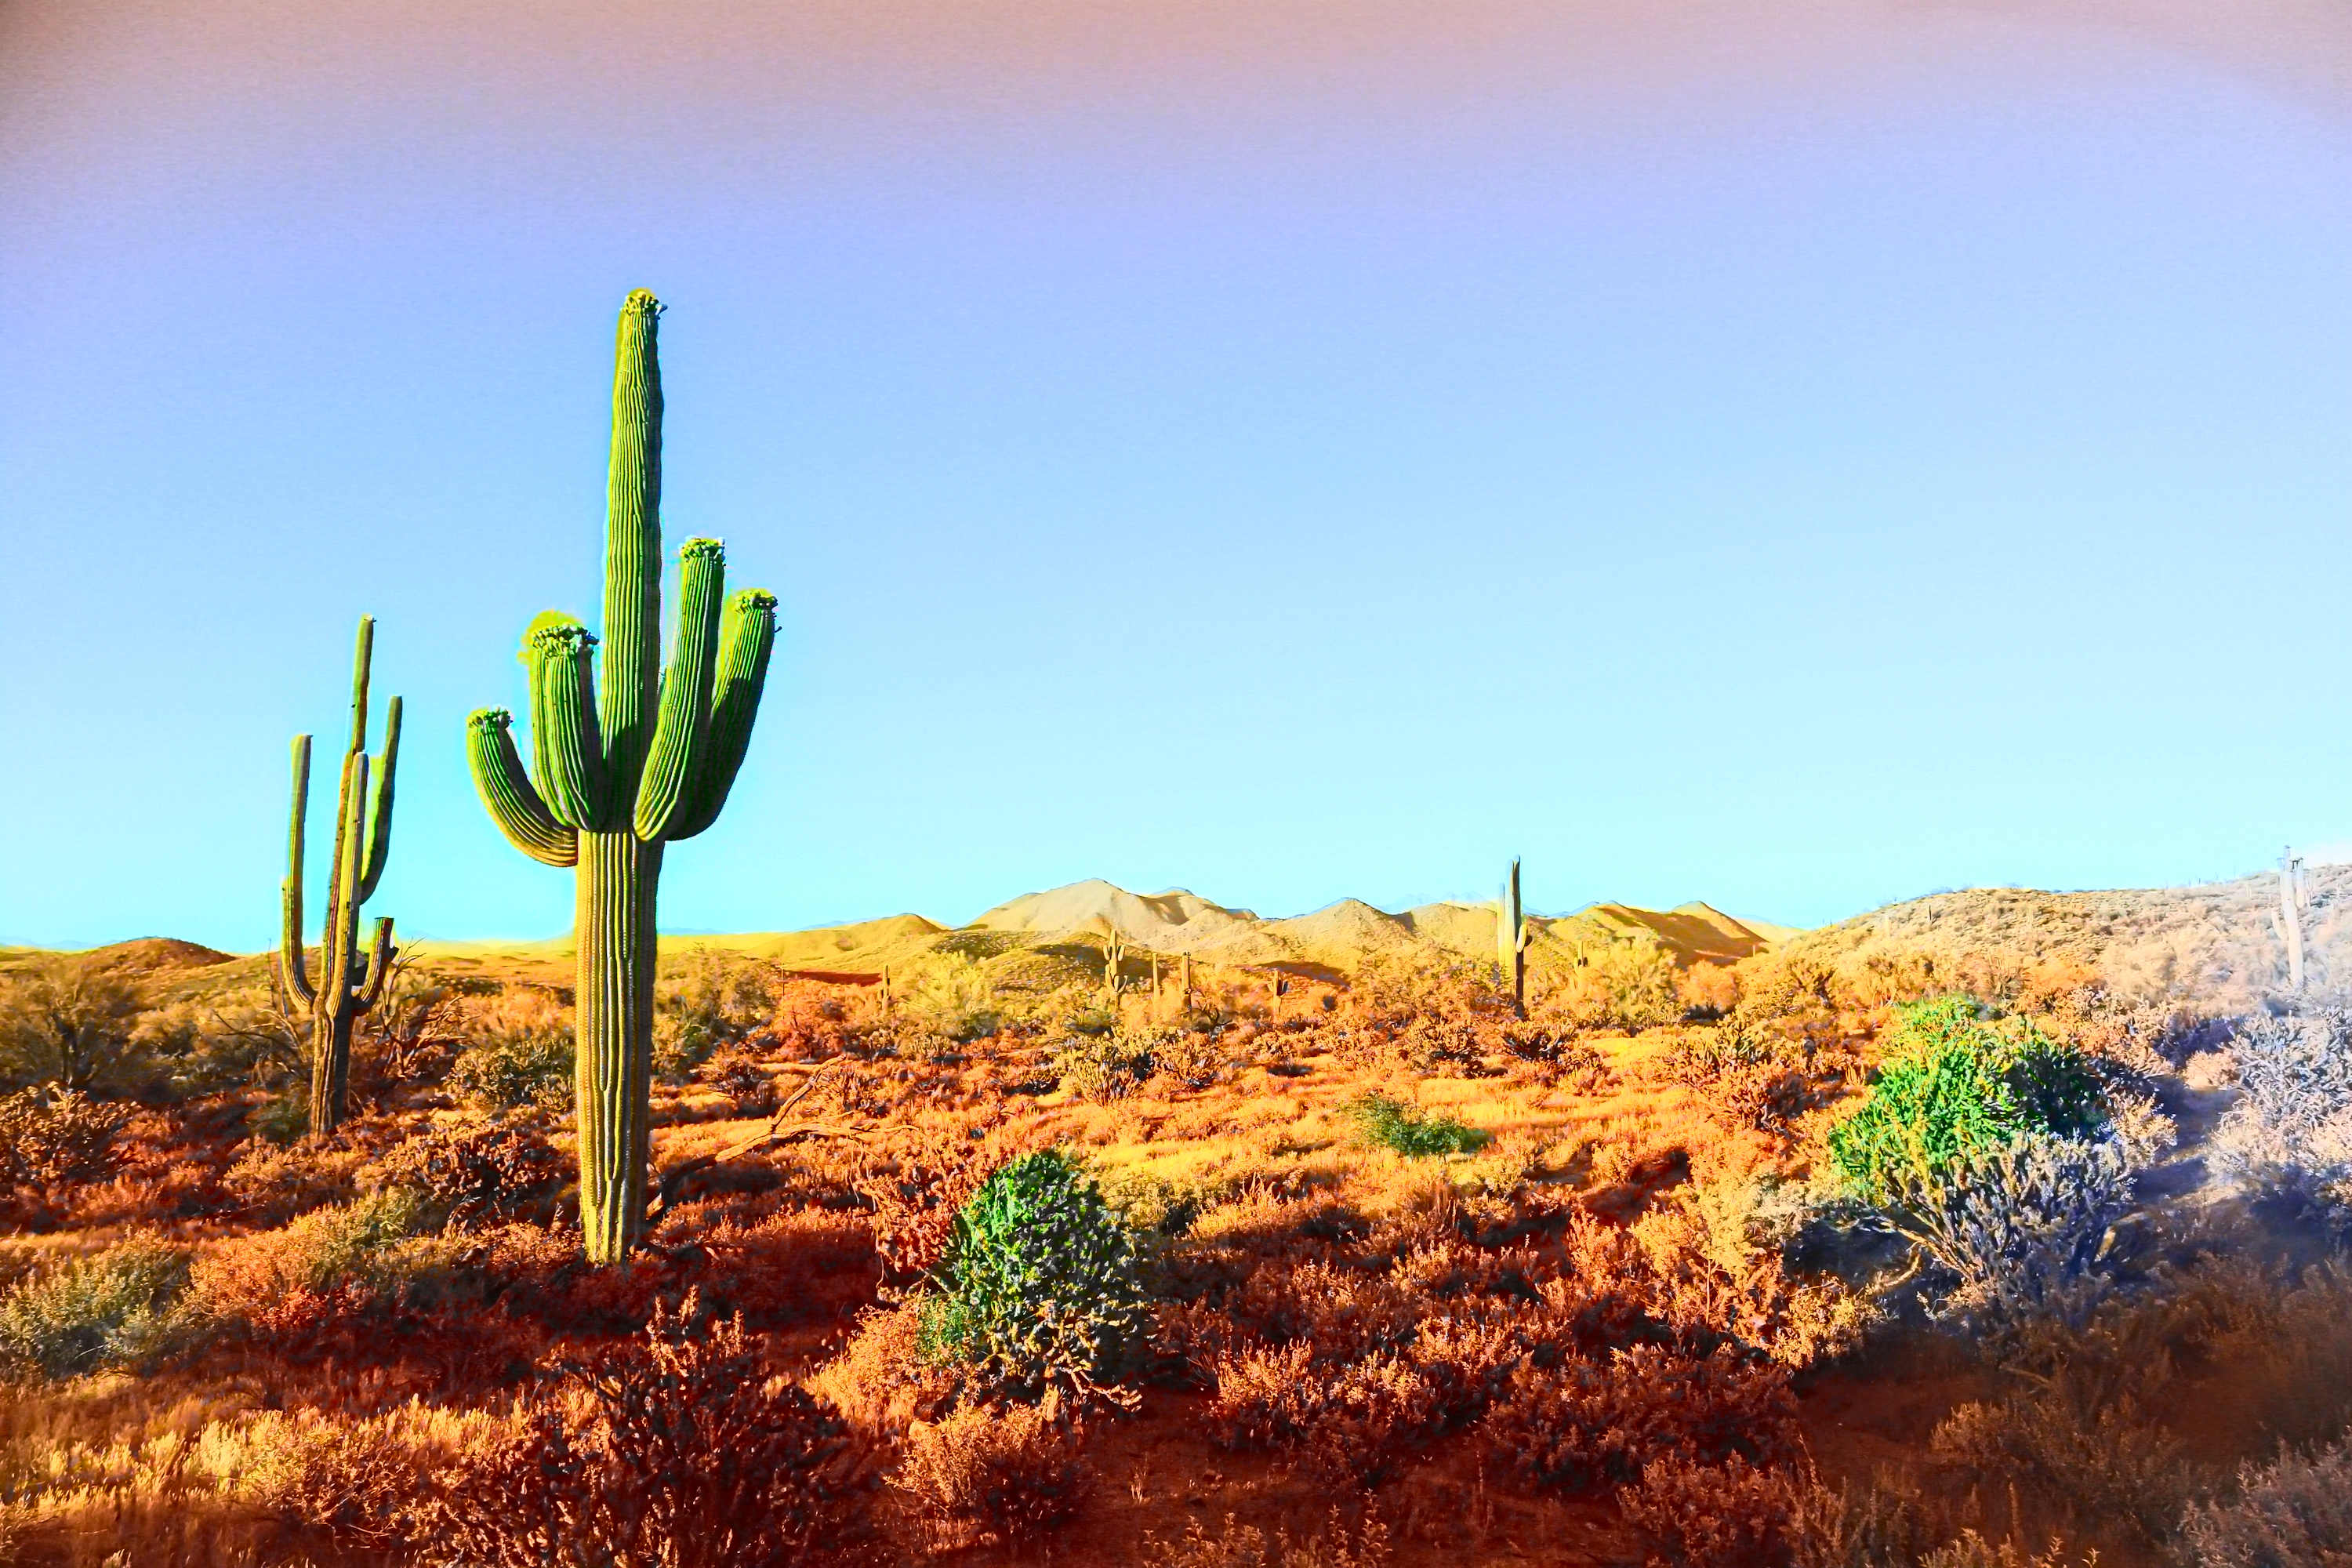
\includegraphics[width=0.19\linewidth]{Figures/step/40.png} &  
    		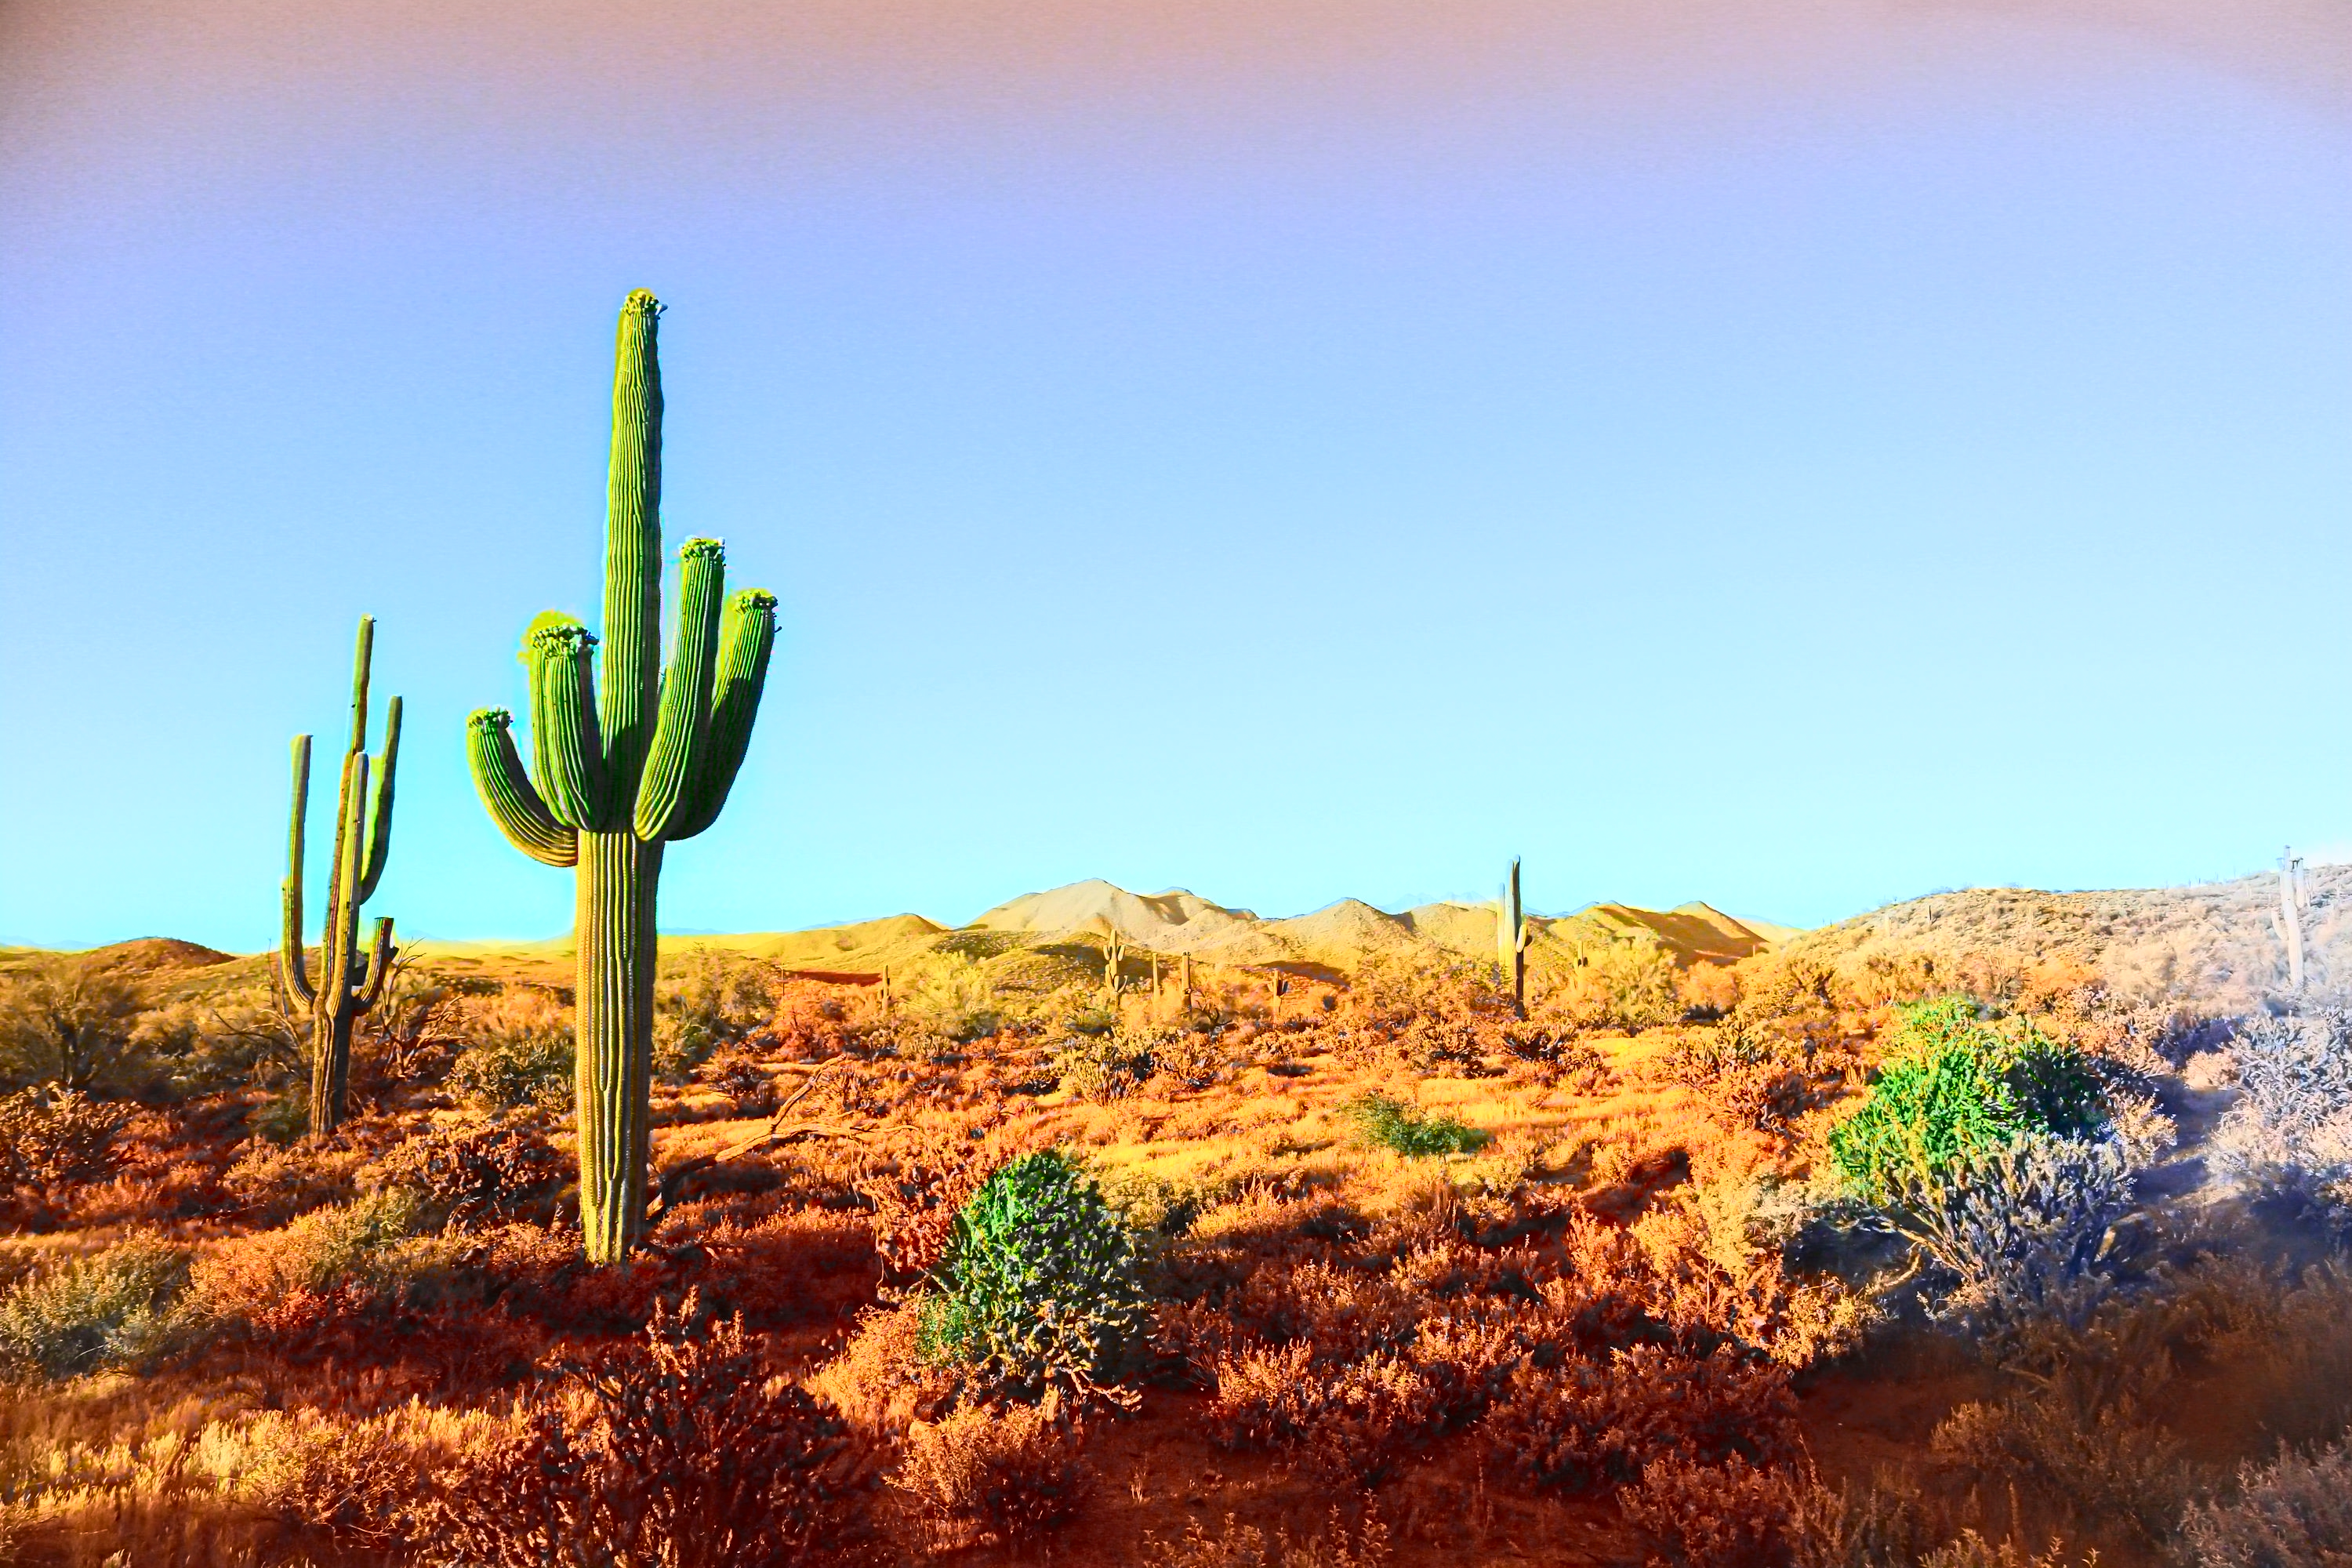
\includegraphics[width=0.19\linewidth]{Figures/step/50.png} \\ [-3pt]   
    		
    		b = 10 & 
    		b = 20 & 
    		b = 30 & 
    		b = 40 & 
    		b = 50 
    		
    	\end{tabular}
    	% \caption{Ảnh so sánh các kết quả khi thay đổi tham số điều chỉnh số bước (b) khử nhiễu của mô hình tô màu.}
    	\label{fig:stepsample}
    \end{figure}
    

\end{frame}

\begin{frame}{Đánh giá sự phụ thuộc của chất lượng ảnh vào các tham số của mô hình (tt)}
    \begin{figure}[htp]
    	\centering
    	\begin{tabular}{@{}c@{\hspace{0.1em}}c@{\hspace{0.1em}}c@{\hspace{0.1em}}c@{}}
    		\includegraphics[width=0.23\linewidth]{Figures/strength/0.5.png} & 
    		\includegraphics[width=0.23\linewidth]{Figures/strength/1.png} & 
    		\includegraphics[width=0.23\linewidth]{Figures/strength/1.5.png} & 
    		\includegraphics[width=0.23\linewidth]{Figures/strength/2.png} \\ [-3pt]   
    		
    		cđ = 0.5 & 
    		cđ = 1 & 
    		cđ = 1.5 & 
    		cđ = 2 
    		
    	\end{tabular}
    	% \caption{Ảnh so sánh các kết quả khi thay đổi giá trị của hệ số điều chỉnh cường độ (cđ) điều khiển của ảnh độ xám.}
    	\label{fig:strsample}
    \end{figure}

\end{frame}
\begin{frame}{Đánh giá độ lem màu}
    \begin{figure}[htp]
    	\centering
    	\begin{tabular}{@{}c@{\hspace{0.1em}}c@{\hspace{0.1em}}c@{\hspace{0.1em}}@{}}
    		\includegraphics[width=0.3\linewidth]{Figures/devae/1.jpg} & 
    		\includegraphics[width=0.3\linewidth]{Figures/devae/novae1.png} &  
    		\includegraphics[width=0.3\linewidth]{Figures/devae/vae1.png} \\ [-3pt] 
    		\includegraphics[width=0.3\linewidth]{Figures/devae/2.jpg} &   
    		\includegraphics[width=0.3\linewidth]{Figures/devae/novae2.png} &  
    		\includegraphics[width=0.3\linewidth]{Figures/devae/vae2.png} \\ 
    		
    		Ảnh gốc &
    		(a) Không sử dụng & 
    		(b) Có sử dụng 
    		
    	\end{tabular}
    	% \caption{Ảnh minh họa so sánh kết quả của mô hình tô màu khi có sử dụng bộ giải mã biến dạng và khi không sử dụng.}
    	\label{fig:devaesample}
    \end{figure}

\end{frame}
